\documentclass{beamer}
\usetheme{Madrid}
\usecolortheme{beaver}
\usepackage{tikz}
\usepackage{amsmath,amssymb}
\usepackage{hyperref}
\usepackage{graphicx}
\usepackage{ulem}
\usetikzlibrary{positioning} % <-- This fixes the 'of' error


\newcommand{\dijkstra}[6]{
\begin{center}
\begin{tikzpicture}[scale=1,
  graphNode/.style={circle, draw, fill=blue!20, minimum size=8mm, inner sep=0pt, font=\bfseries},
  aboveLabel/.style={rectangle, draw=green!60!black, fill=green!20, font=\small, minimum height=4mm},
  edgeLabel/.style={font=\small}
]

% Nodes with green boxed labels
\node[graphNode] (T) at (0,0) {T};
\node[aboveLabel, above=2pt of T] {0};

\node[graphNode] (E) at (2,-2) {E};
\node[aboveLabel, above=2pt of E] {#5};

\node[graphNode] (A) at (2,1) {A};
\node[aboveLabel, above=2pt of A] {#4};

\node[graphNode] (NB) at (4,2) {NB};
\node[aboveLabel, above=2pt of NB] {#3};

\node[graphNode] (MR) at (4,0) {MR};
\node[aboveLabel, above=2pt of MR] {#2};

\node[graphNode] (P) at (4,-1) {P};
\node[aboveLabel, below=2pt of P] {#1};

\node[graphNode] (Y) at (8,0) {Y};
\node[aboveLabel, above=2pt of Y] {#6};

% Edges with plain text labels
\draw (T) -- (E) node[midway, left, edgeLabel] {57};
\draw (T) -- (A) node[midway, left, edgeLabel] {20};
\draw (A) -- (NB) node[midway, left, edgeLabel] {36};
\draw (NB) -- (Y) node[midway, above, edgeLabel] {120};
\draw (E) -- (P) node[midway, below, edgeLabel] {27};
\draw (P) -- (Y) node[midway, below, edgeLabel] {76};
\draw (A) -- (MR) node[midway, above, edgeLabel] {79};
\draw (MR) -- (P) node[midway, left, edgeLabel] {10};
\draw (MR) -- (Y) node[midway, above, edgeLabel] {90};
\end{tikzpicture}
\end{center}
}

\newcommand{\ph}{\phantom{$\infty$}}

\title{Shortest Path Algorithms}
\author{Graph Theory}
\date{\today}

\begin{document}

\begin{frame}
\titlepage

\begin{center}
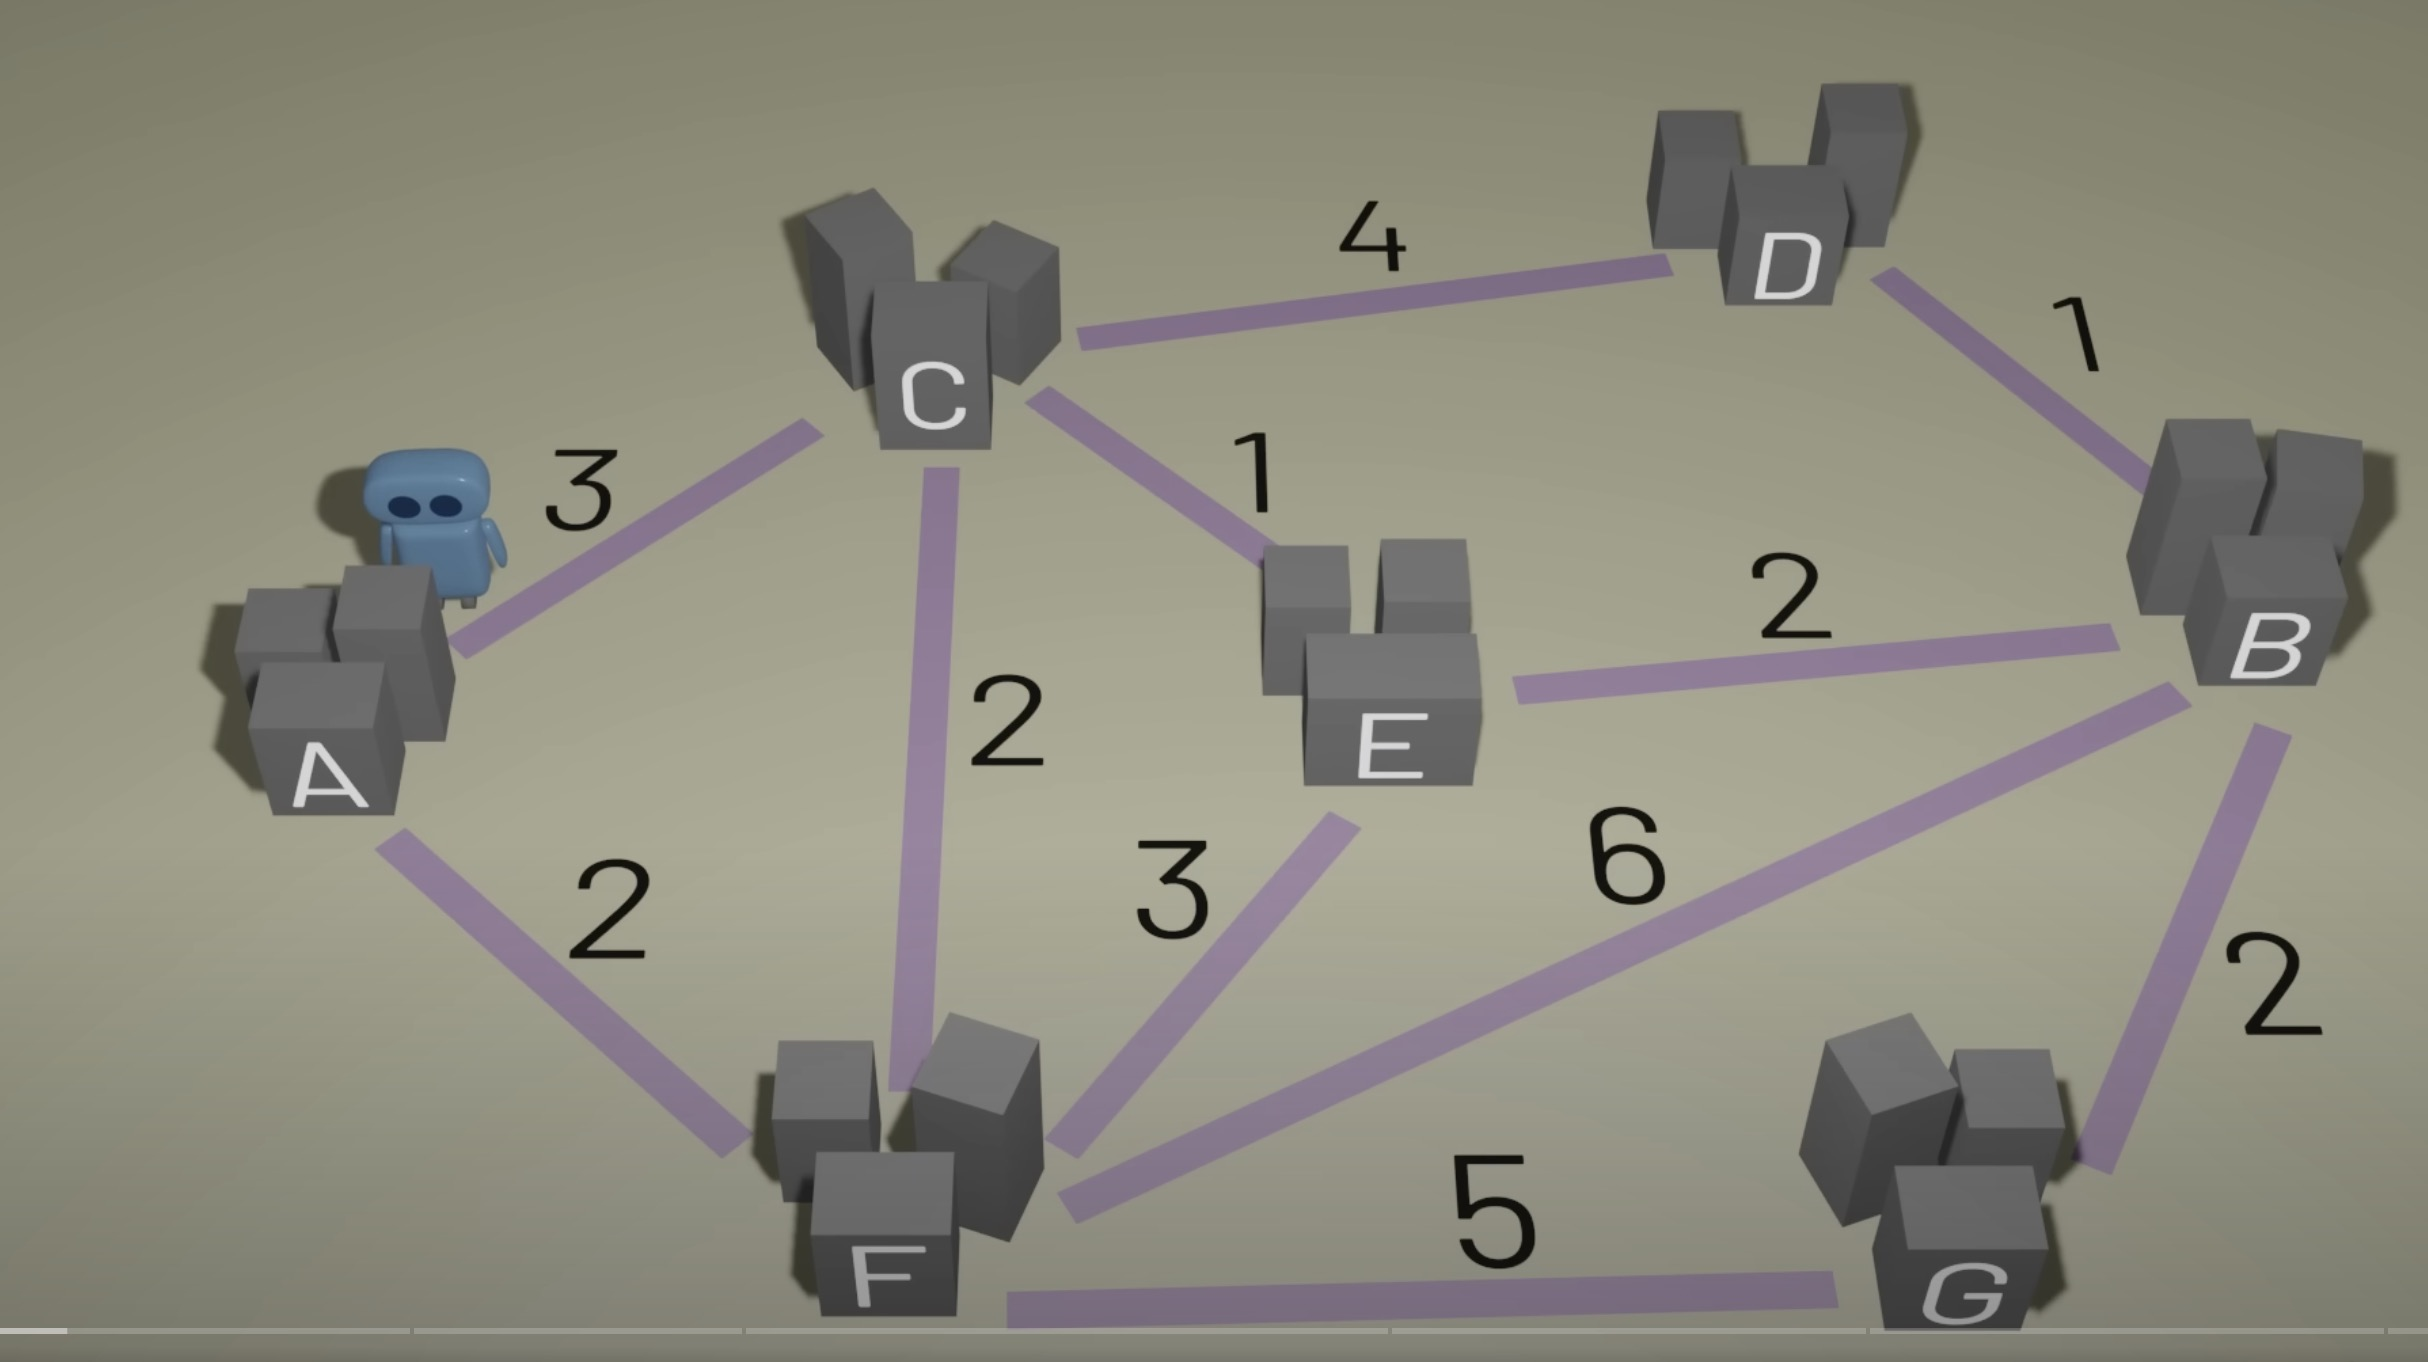
\includegraphics[scale = 0.08]{Figures/dijkstra-video}
\end{center}
\end{frame}

\begin{frame}{Outline}
\begin{itemize}
\item Video
\item Problem Statement
\item Dijkstra's Algorithm
\item Examples
\item Efficiency
\item Software Solutions
\end{itemize}
\end{frame}
\begin{frame}{Video}
\url{https://www.youtube.com/watch?v=EFg3u_E6eHU&ab_channel=SpanningTree}\\
\textbf{How Dijkstra's Algorithms Works} by Spanning Tree

\end{frame}

\begin{frame}{Problem Statement}
\begin{itemize}
\item When using applications like Google Maps, you're looking for a \textbf{shortest path}
\item The street maps are represented as graphs
\item Edge weights represent estimated driving times
\item While simple cases can be solved by guess-and-check, we need systematic approaches for complex problems
\item We need \textbf{algorithms} - step-by-step procedures for solving problems
\end{itemize}
\end{frame}


\begin{frame}{Shortest Path Problem: Definition}
\begin{block}{The Shortest Path Problem}
Given a network $G = (V, A)$ with costs $c_{ij}$ on the arcs, find the path from a source node $s$ to a target node $t$ that minimizes the total cost.
\end{block}

\begin{block}{Sets}
\begin{itemize}
\item $V$: Set of nodes in the network
\item $A$: Set of arcs in the network
\end{itemize}
\end{block}

\begin{block}{Parameters}
\begin{itemize}
\item $c_{ij}$: Cost (or distance) of traversing arc $(i,j) \in A$
\item $s$: Source node
\item $t$: Target node
\end{itemize}
\end{block}

\begin{block}{Variables}
\begin{itemize}
\item $x_{ij}$: flow along arc $(i,j)$ on the shortest path
\end{itemize}
\end{block}
\end{frame}

\begin{frame}{Shortest Path Problem: Mathematical Model}
\begin{block}{Objective Function}
Minimize the total cost of the selected path:
\begin{align*}
\text{Minimize} \quad \sum_{(i,j) \in A} c_{ij} x_{ij}
\end{align*}
\end{block}

\begin{block}{Constraints}
Flow Conservation:
\begin{align*}
\sum_{j:(i,j) \in A} x_{ij} - \sum_{j:(j,i) \in A} x_{ji} = 
\begin{cases} 
1 & \text{if } i = s \\
-1 & \text{if } i = t \\
0 & \text{otherwise}
\end{cases}
\quad \forall i \in V
\end{align*}

Non-negativity Constraints:
\begin{align*}
x_{ij} 
\geq 0 \quad \forall (i,j) \in A
\end{align*}
\end{block}
\end{frame}
\begin{frame}
\begin{block}{Applications}
\begin{itemize}
\item Route planning
\item Network routing
\item Logistics optimization
\item Social network analysis
\end{itemize}
\end{block}
\end{frame}


\begin{frame}{Dijkstra's Algorithm}
\begin{enumerate}
\item Mark the starting vertex with a distance of zero. Designate this vertex as current.
\item Find all vertices leading to the current vertex. Calculate their distances to the start.
\item Mark the current vertex as visited. We will never look at this vertex again.
\item Mark the vertex with the smallest distance as current, and repeat from step 2.
\end{enumerate}
\end{frame}

\begin{frame}
\begin{center}
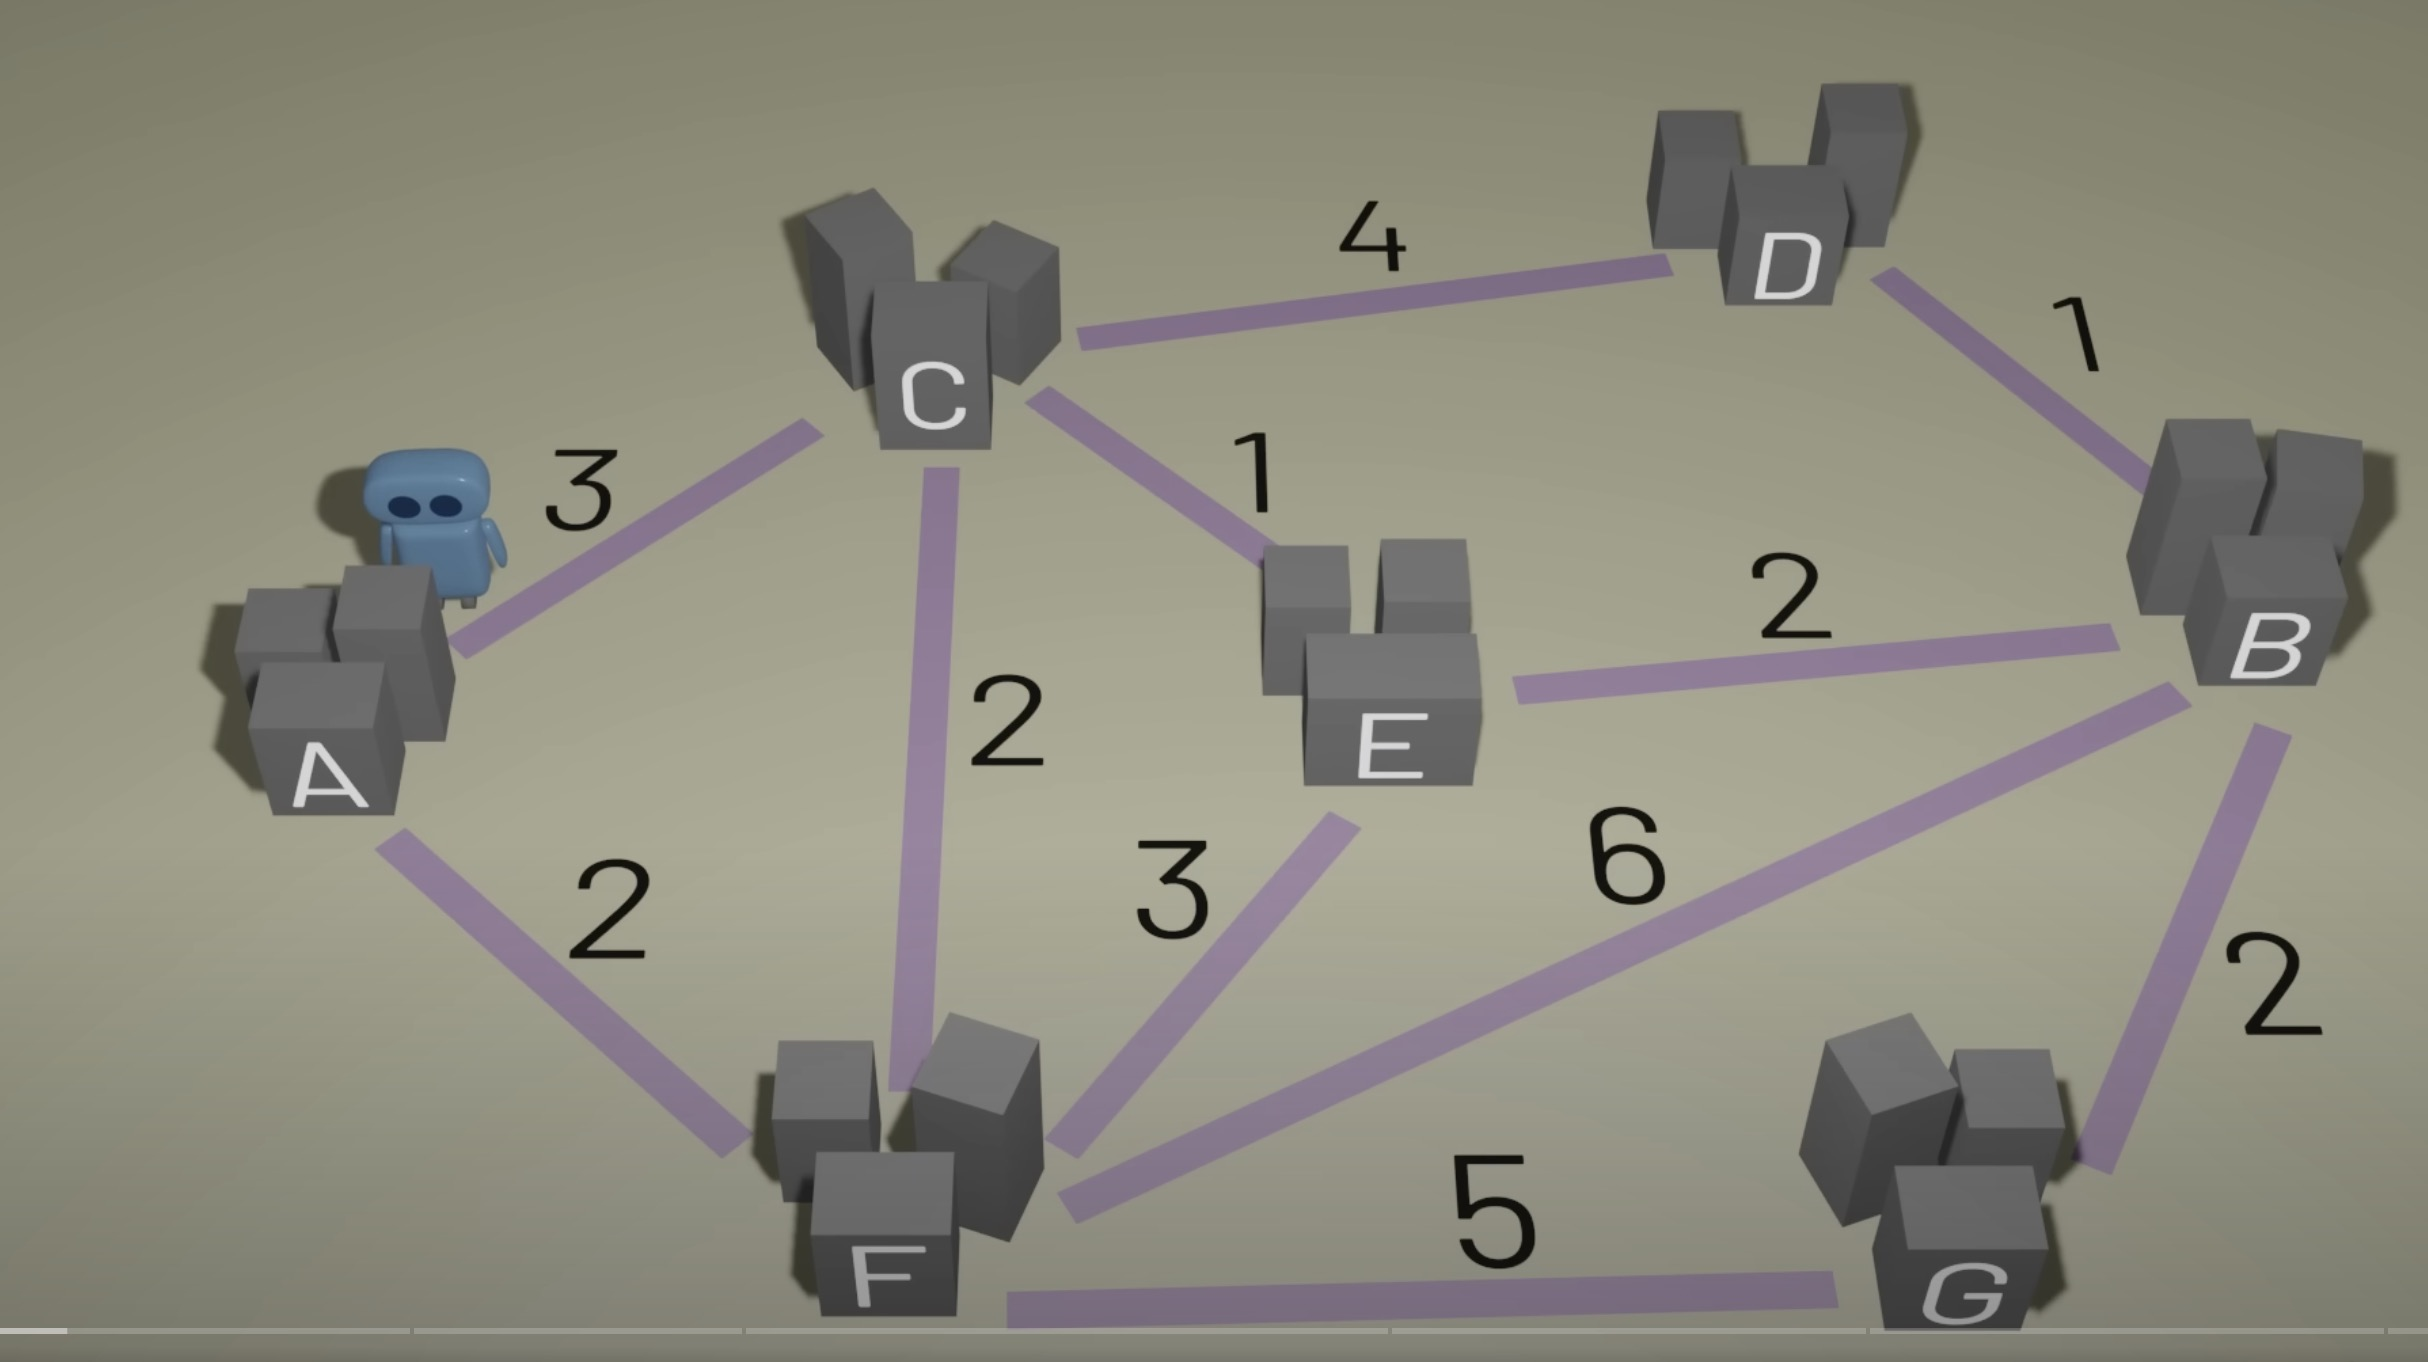
\includegraphics[scale = 0.13]{Figures/dijkstra-video}\\
\href{https://www.youtube.com/watch?v=EFg3u_E6eHU}{How Dijkstra's algorithm works (YouTube)}
\end{center}
\end{frame}

\begin{frame}
\begin{center}
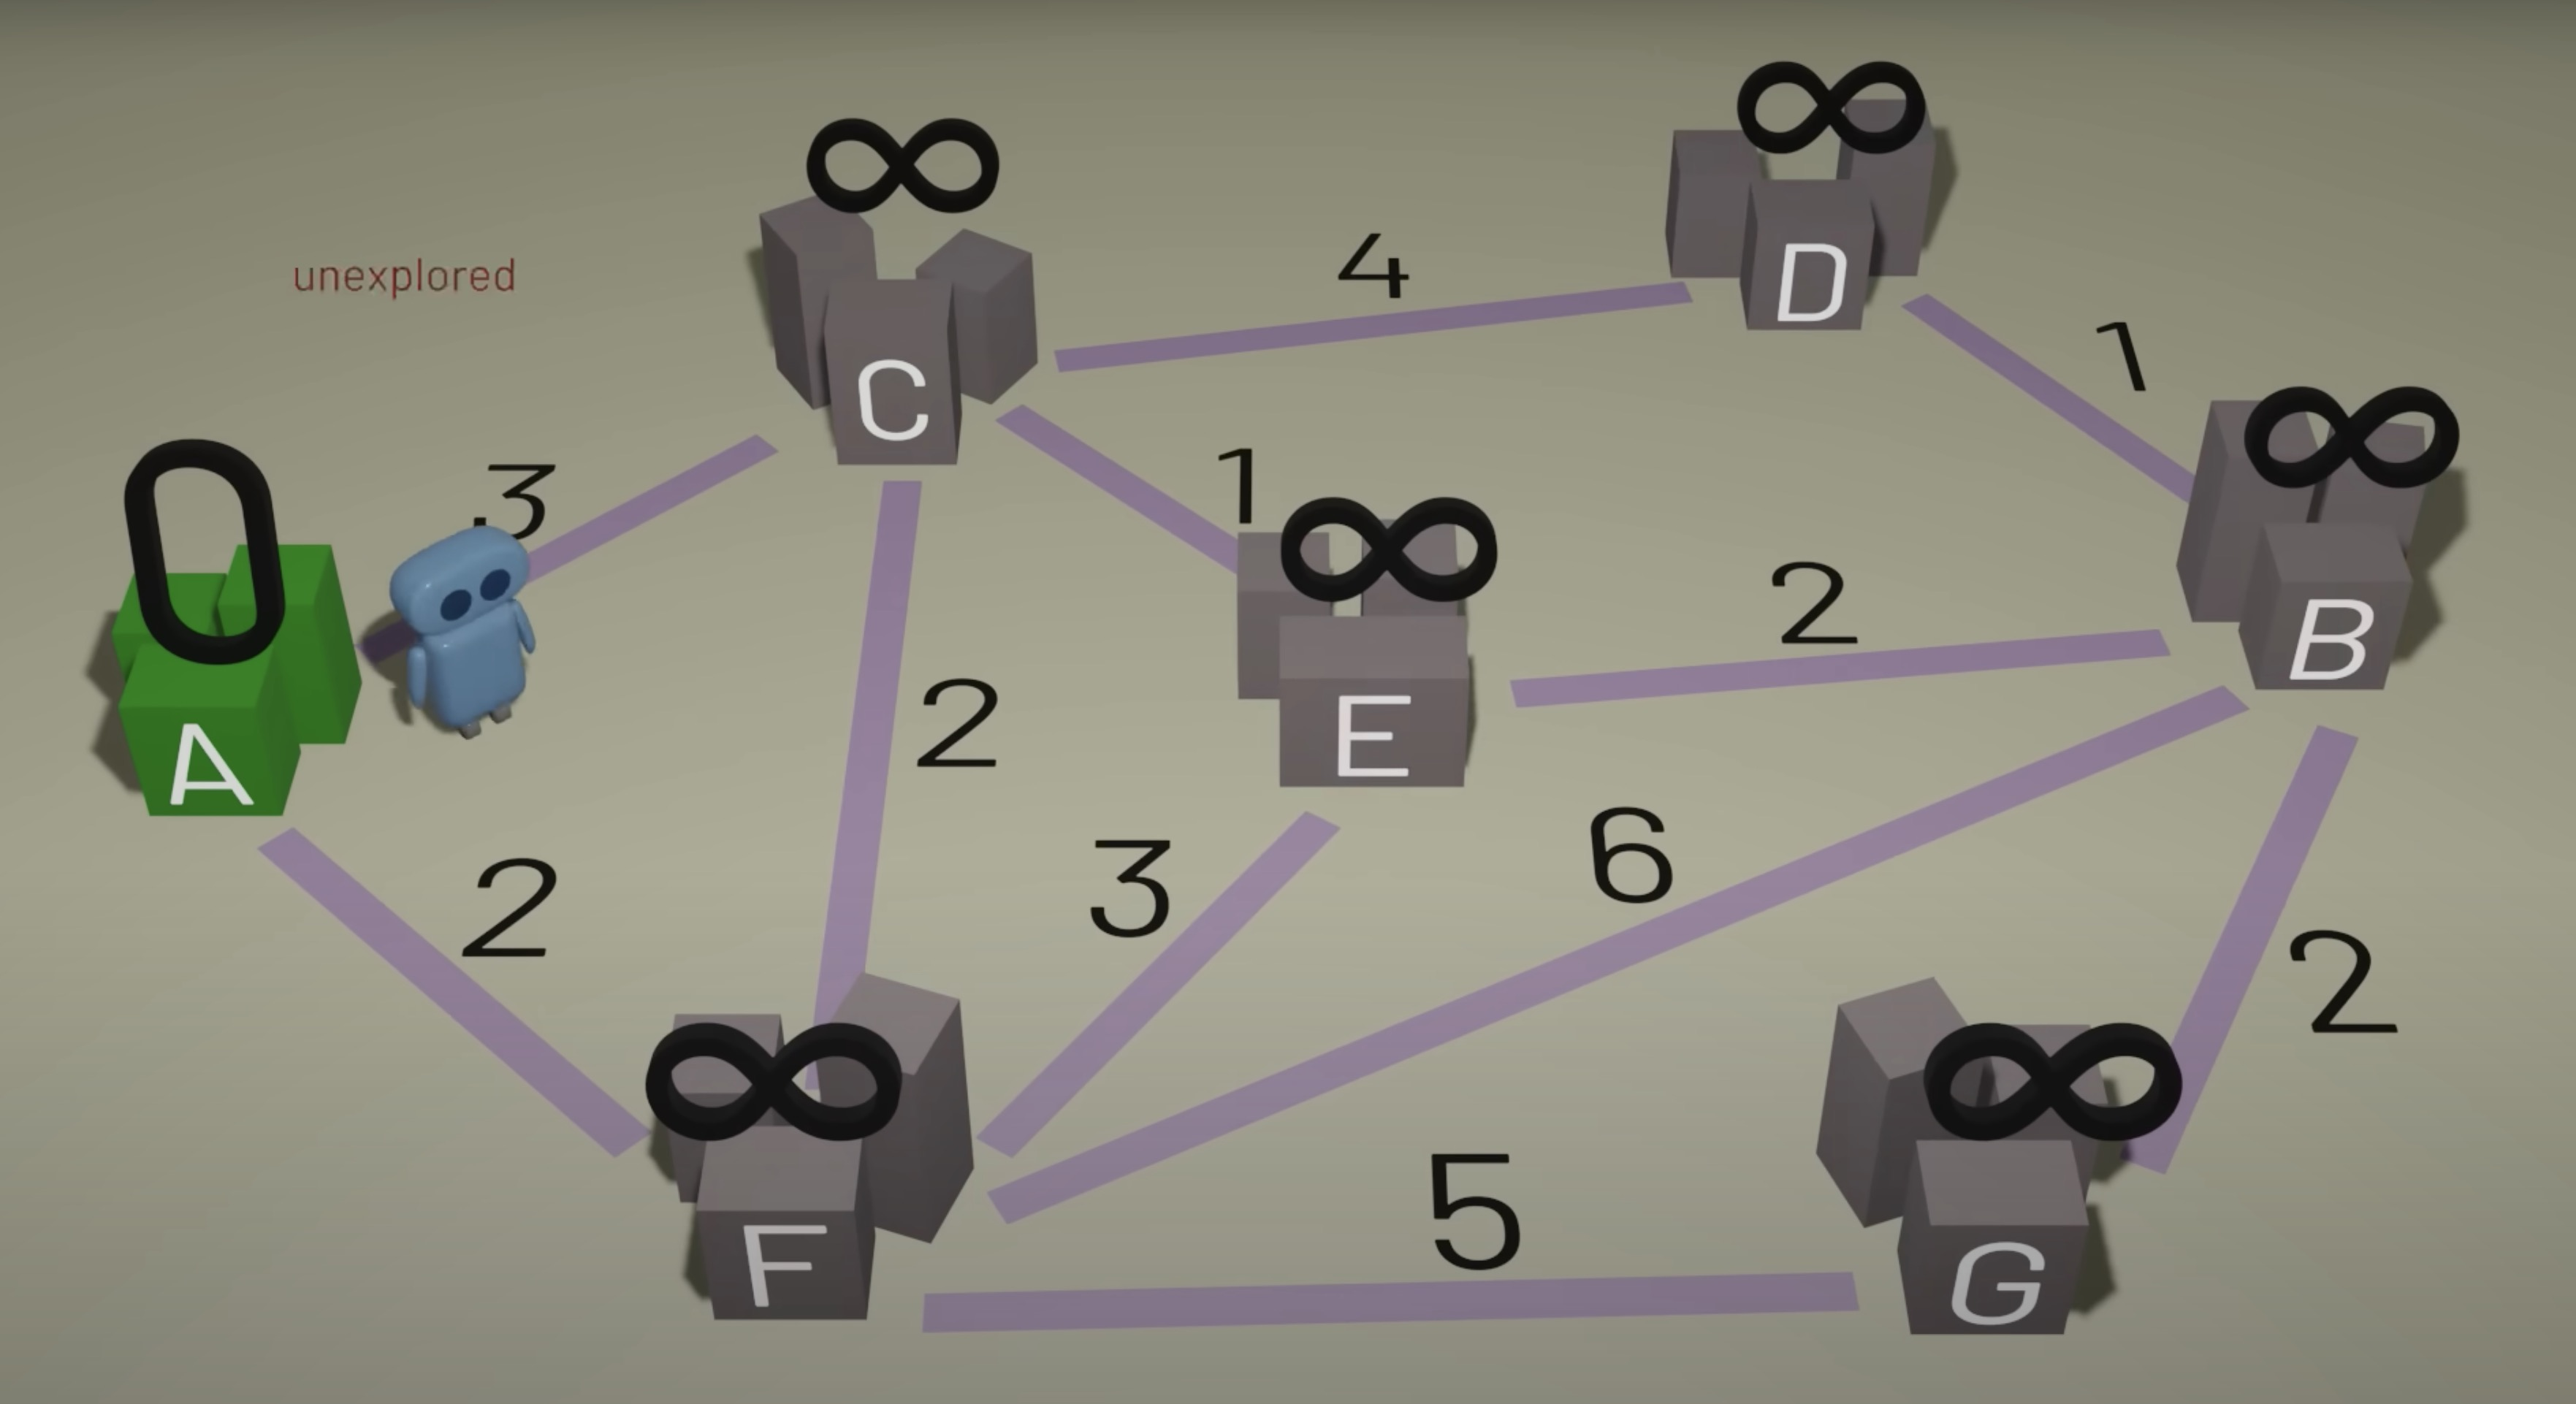
\includegraphics[scale = 0.07]{Figures/dijkstra-video-start}\\
\begin{tabular}{|l|l|l|l|l|l|l|l|}
\hline
current & a & f&c&e&d&g&b \\ \hline
&&&&&&& \\ \hline
&&&&&&& \\ \hline
&&&&&&& \\ \hline
&&&&&&& \\ \hline
&&&&&&& \\ \hline
&&&&&&& \\ \hline
\end{tabular}
\end{center}
\end{frame}

\begin{frame}
\begin{center}
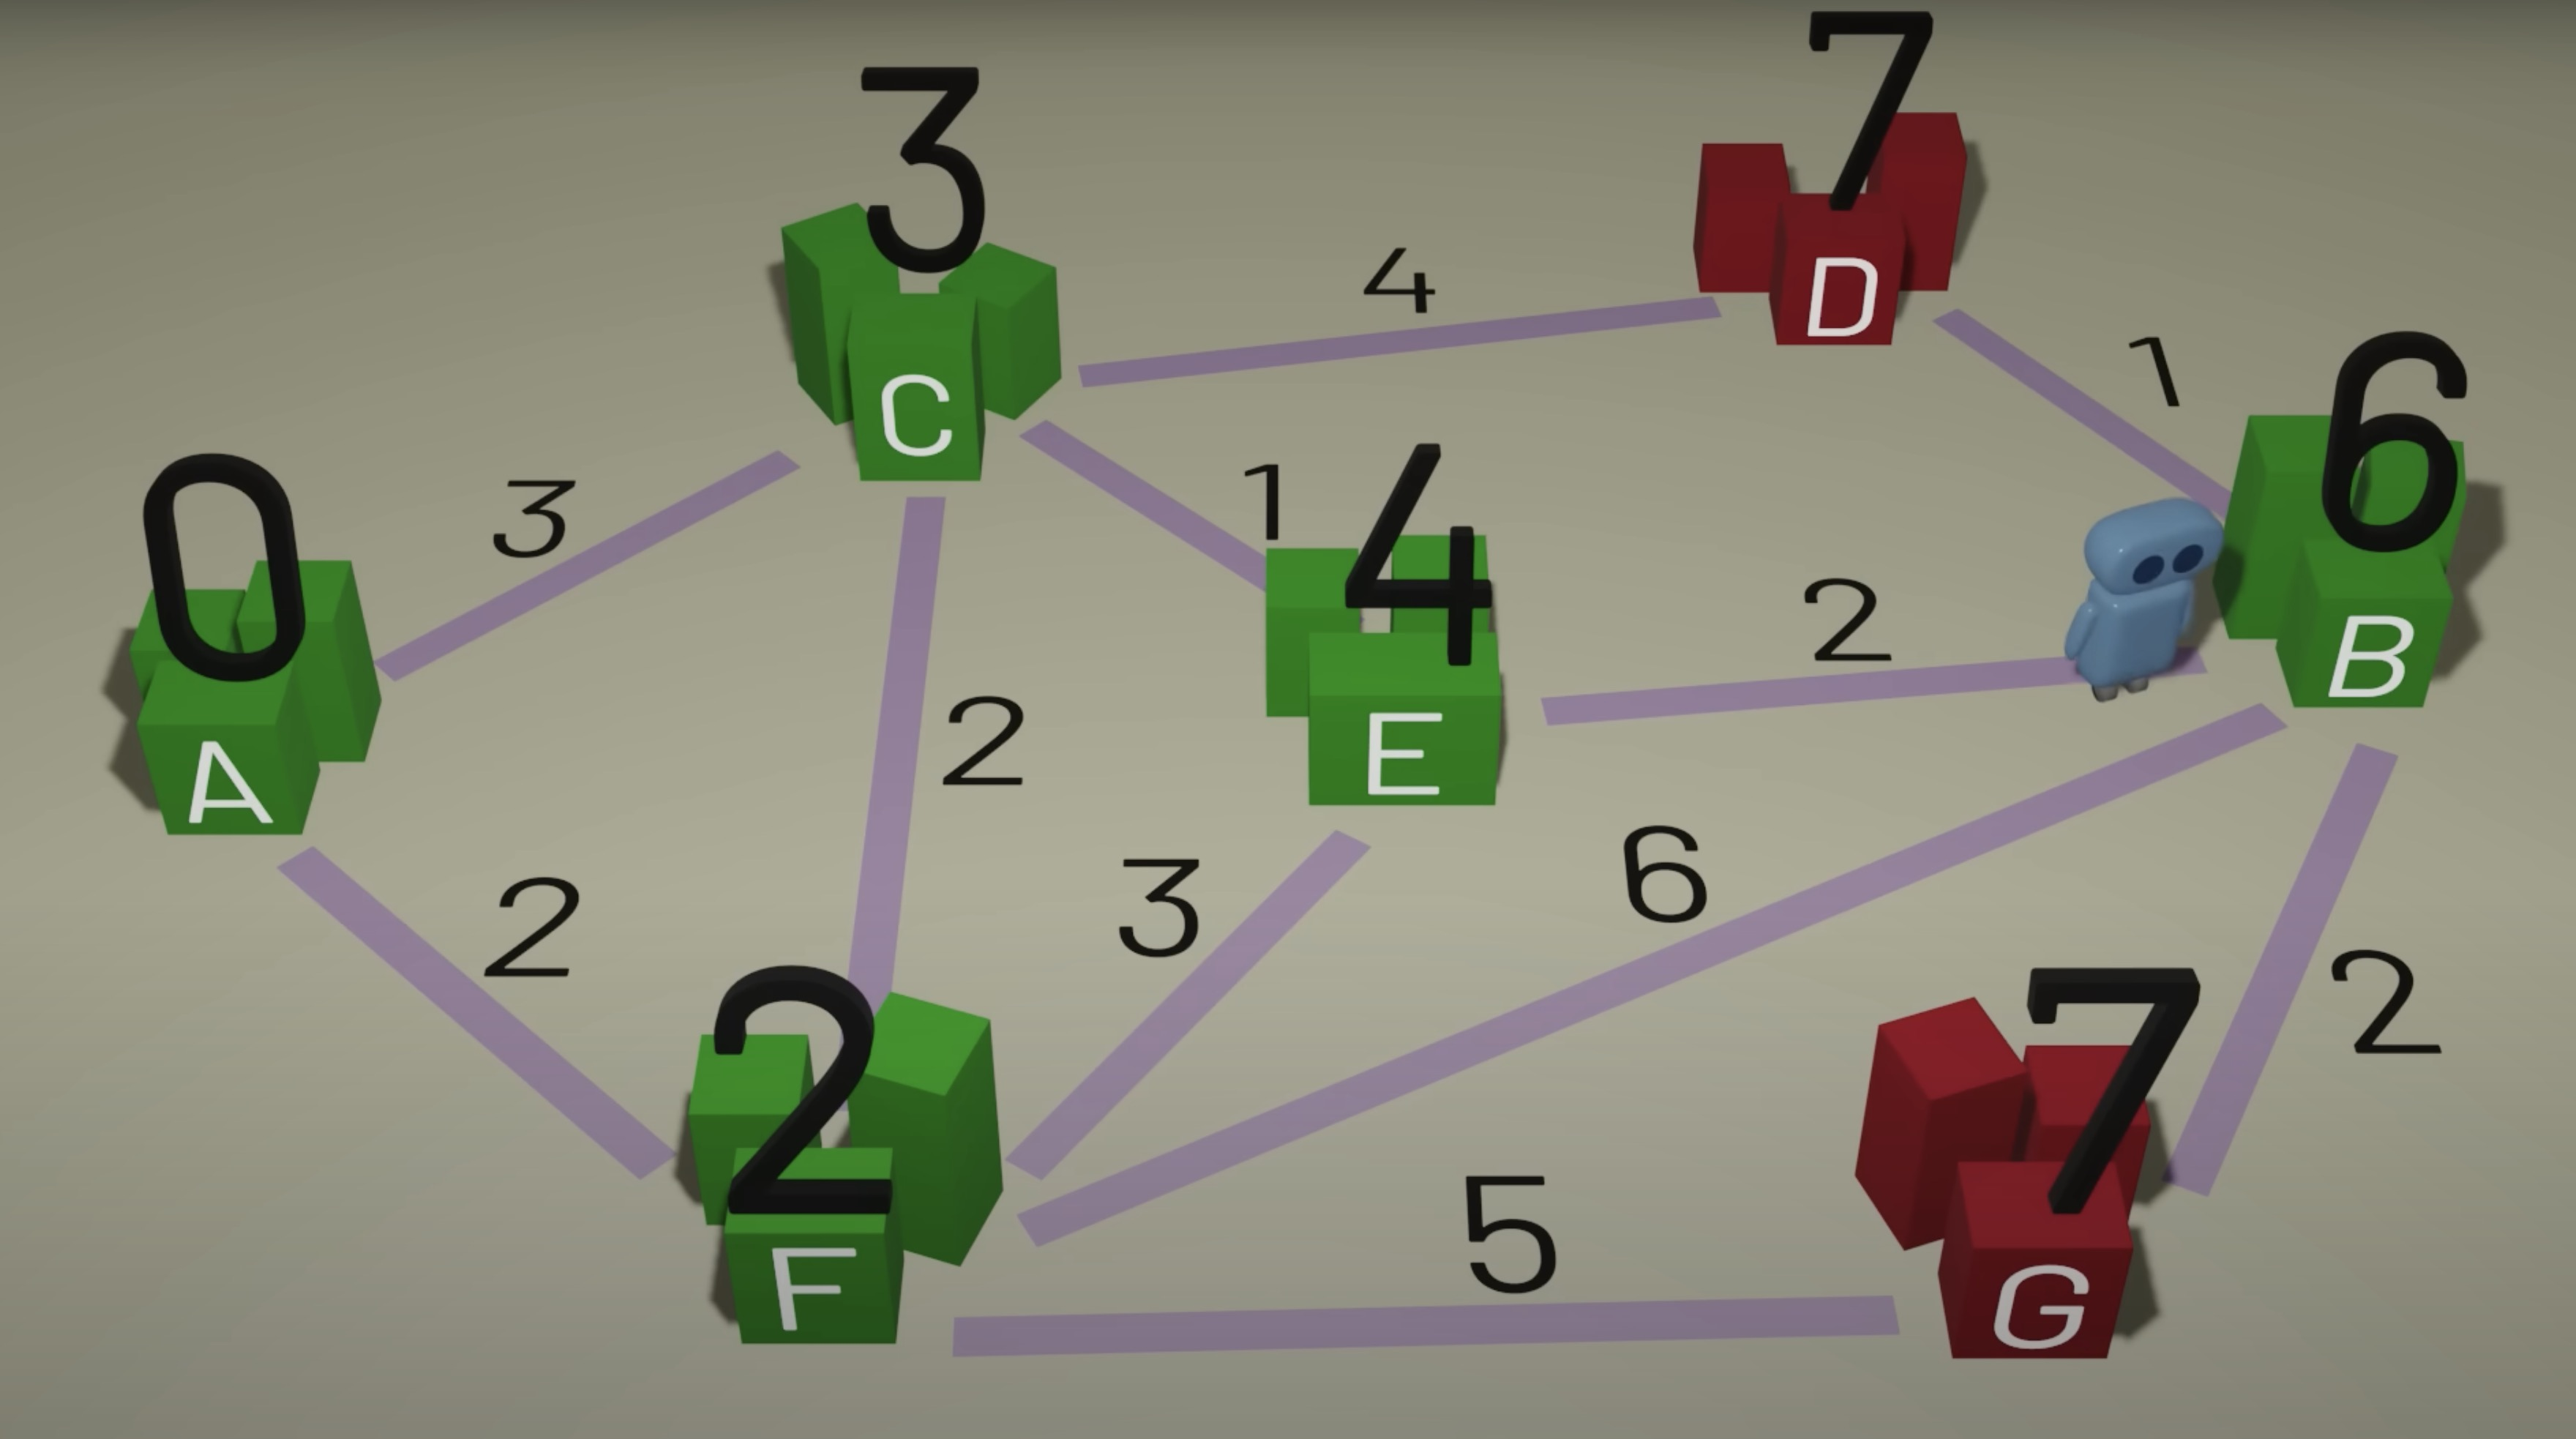
\includegraphics[scale = 0.07]{Figures/dijkstra-video-end}\\
\begin{tabular}{|l|l|l|l|l|l|l|l|}
\hline
current & a & f&c&e&d&g&b \\ \hline
a &0 &2&3&$\infty$&$\infty$&$\infty$&$\infty$ \\ \hline
f &- &-&3&5&$\infty$&7&$\infty$ \\ \hline
c&-&-&-&4&7&7&$\infty$ \\ \hline
e&-&-&-&-&7&7&6 \\ \hline
\end{tabular}
\end{center}
\end{frame}

\begin{frame}{Example 1: Yakima to Tacoma}
\dijkstra{}{}{}{}{}{}

\end{frame}



\begin{frame}{Example 1: Yakima to Tacoma}
\dijkstra{$\infty$}{$\infty$}{$\infty$}{$\infty$}{$\infty$}{$\infty$}
\begin{itemize}
\item Finding shortest path from Tacoma (T) to Yakima (Y)
\item Graph shows travel times in minutes
\end{itemize}
\end{frame}


\begin{frame}{Resources}
\begin{itemize}
\item \href{https://www.youtube.com/watch?v=EFg3u_E6eHU}{How Dijkstra's algorithm works (YouTube)}
\item \href{https://github.com/open-optimization/open-optimization-or-book/blob/master/instructive-code/networkx\%20example\%20-\%20Dijkstra's\%20Algorithm.ipynb}{Python Example using Networkx}
\end{itemize}
\end{frame}

%\begin{frame}
%\begin{center}
%\begin{tikzpicture}[scale=1,
%  graphNode/.style={circle, draw, fill=blue!20, minimum size=8mm, inner sep=0pt, font=\bfseries},
%  aboveLabel/.style={rectangle, draw=green!60!black, fill=green!20, font=\small, minimum height=4mm},
%  edgeLabel/.style={font=\small}
%]
%
%% Nodes with green boxed labels
%\node[graphNode] (T) at (0,0) {T};
%\node[aboveLabel, above=2pt of T] {$\infty$};
%
%\node[graphNode] (E) at (2,-2) {E};
%\node[aboveLabel, above=2pt of E] {$\infty$};
%
%\node[graphNode] (A) at (2,1) {A};
%\node[aboveLabel, above=2pt of A] {$\infty$};
%
%\node[graphNode] (NB) at (4,2) {NB};
%\node[aboveLabel, above=2pt of NB] {$\infty$};
%
%\node[graphNode] (MR) at (4,0) {MR};
%\node[aboveLabel, above=2pt of MR] {$\infty$};
%
%\node[graphNode] (P) at (4,-1) {P};
%\node[aboveLabel, below=2pt of P] {$\infty$};
%
%\node[graphNode] (Y) at (8,0) {Y};
%\node[aboveLabel, above=2pt of Y] {$0$};
%
%% Edges with plain text labels
%\draw (T) -- (E) node[midway, left, edgeLabel] {57};
%\draw (T) -- (A) node[midway, left, edgeLabel] {20};
%\draw (A) -- (NB) node[midway, left, edgeLabel] {36};
%\draw (NB) -- (Y) node[midway, above, edgeLabel] {104};
%\draw (E) -- (P) node[midway, below, edgeLabel] {96};
%\draw (P) -- (Y) node[midway, below, edgeLabel] {76};
%\draw (A) -- (MR) node[midway, above, edgeLabel] {79};
%\draw (MR) -- (P) node[midway, left, edgeLabel] {21};
%\draw (MR) -- (Y) node[midway, above, edgeLabel] {102};
%
%\end{tikzpicture}
%\end{center}


%\end{frame}

\begin{frame}
\dijkstra{\ph}{\ph}{\ph}{\ph}{\ph}{\ph}
\begin{center}
\begin{tabular}{|l|l|l|l|l|l|l|l|}
\hline
current & T & A & E & NB & MR & P & Y \\ \hline
&&&&&&& \\ \hline
&&&&&&& \\ \hline
&&&&&&& \\ \hline
&&&&&&& \\ \hline
&&&&&&& \\ \hline
&&&&&&& \\ \hline
\end{tabular}
\end{center}
\end{frame}


\begin{frame}
\begin{columns}
\begin{column}{0.7\textwidth}
\dijkstra{\ph}{\ph}{\ph}{\ph}{\ph}{\ph}
\begin{center}
\begin{tabular}{|l|l|l|l|l|l|l|l|}
\hline
current & T & A & E & NB & MR & P & Y \\ \hline
&&&&&&& \\ \hline
&&&&&&& \\ \hline
&&&&&&& \\ \hline
&&&&&&& \\ \hline
&&&&&&& \\ \hline
&&&&&&& \\ \hline
\end{tabular}
\end{center}
\end{column}
\begin{column}{0.3\textwidth}
\begin{enumerate}
\item starting vertex = current, dist = 0.
\item Find all leading to the current vertex. Calculate distances to the start.
\item Mark the current vertex as visited. We will never look at this vertex again.
\item Mark  vertex with  smallest distance as current, and repeat  2.
\end{enumerate}
\end{column}
\end{columns}
\end{frame}



\begin{frame}
\dijkstra{\ph}{\ph}{\ph}{\ph}{\ph}{\ph}
\begin{center}
\begin{tabular}{|l|l|l|l|l|l|l|l|}
\hline
current & T & A & E & NB & MR & P & Y \\ \hline
&&&&&&& \\ \hline
\end{tabular}
\end{center}
\end{frame}
\begin{frame}
\dijkstra{\ph}{\ph}{\ph}{\ph}{\ph}{\ph}
\begin{center}
\begin{tabular}{|l|l|l|l|l|l|l|l|}
\hline
current & T & A & E & NB & MR & P & Y \\ \hline
&&&&&&& \\ \hline
\end{tabular}
\end{center}
\end{frame}
\begin{frame}
\dijkstra{\ph}{\ph}{\ph}{\ph}{\ph}{\ph}
\begin{center}
\begin{tabular}{|l|l|l|l|l|l|l|l|}
\hline
current & T & A & E & NB & MR & P & Y \\ \hline
&&&&&&& \\ \hline
\end{tabular}
\end{center}
\end{frame}
\begin{frame}
\dijkstra{\ph}{\ph}{\ph}{\ph}{\ph}{\ph}
\begin{center}
\begin{tabular}{|l|l|l|l|l|l|l|l|}
\hline
current & T & A & E & NB & MR & P & Y \\ \hline
&&&&&&& \\ \hline
\end{tabular}
\end{center}
\end{frame}

\begin{frame}
\dijkstra{\ph}{\ph}{\ph}{\ph}{\ph}{\ph}
\begin{center}
\begin{tabular}{|l|l|l|l|l|l|l|l|}
\hline
current & T & A & E & NB & MR & P & Y \\ \hline
&&&&&&& \\ \hline
\end{tabular}
\end{center}
\end{frame}


\begin{frame}
\dijkstra{\ph}{\ph}{\ph}{\ph}{\ph}{\ph}
\begin{center}
\begin{tabular}{|l|l|l|l|l|l|l|l|}
\hline
current & T & A & E & NB & MR & P & Y \\ \hline
&&&&&&& \\ \hline
\end{tabular}
\end{center}
\end{frame}

\begin{frame}
\begin{center}
\begin{tabular}{|l|l|l|l|l|l|l|l|}
\hline
current & T & A & E & NB & MR & P & Y \\ \hline
&&&&&&& \\ \hline
&&&&&&& \\ \hline
&&&&&&& \\ \hline
&&&&&&& \\ \hline
&&&&&&& \\ \hline
&&&&&&& \\ \hline
\end{tabular}
\end{center}
\end{frame}



%\begin{frame}{Example 1: Step 1}
%
%\dijkstra{$\infty$}{$\infty$ }{ $\infty$}{$\infty$ }{$\infty$ }{$\infty$ }
%
%\begin{itemize}
%\item Mark the ending vertex (Y) with a distance of zero
%\item Designate Y as current
%\end{itemize}
%\end{frame}
%
%\begin{frame}{Example 1: Step 2}
%
%\dijkstra{76}{102 }{ 104}{$\infty$ }{$\infty$ }{$\infty$ }{$\infty$ }
%
%\begin{itemize}
%\item Calculate distances for vertices leading to Y
%\item NB: 104 minutes from end, 
%MR: 102 minutes from end, 
%P: 76 minutes from end
%\end{itemize}
%\end{frame}
%
%\begin{frame}{Example 1: Steps 3 \& 4}
%\begin{center}
%\begin{tikzpicture}[scale=0.7]
%\draw[fill] (0,0) circle[radius=.1] node[left]{T};
%\draw[fill] (2,-2) circle[radius=.1] node[left]{E\textcolor{red}{[172]}};
%\draw[fill] (2,1) circle[radius=.1];
%\node at (1.5,1.2){A\textcolor{red}{[175]}};
%\draw[fill] (4,2) circle[radius=.1]; 
%\node at (3.6,2.3){NB\textcolor{red}{[104]}};
%\draw[fill] (4,0) circle[radius=.1];
%\node at (4.3,0.3){MR\textcolor{red}{[96]}};
%\draw[fill] (4,-1) circle[radius=.1];
%\node at (4.6,-1.2){\textcolor{gray}{\sout{P}}\textcolor{red}{[76]}};
%\draw[fill] (8,0) circle[radius=.1] node[right]{\textcolor{gray}{\sout{Y}}\textcolor{red}{[0]}};
%\draw(0,0)--(2,-2);
%\node at (0.6,-1){57};
%\draw(0,0)--(2,1);
%\node at (0.5, 0.5){20};
%\draw(2,1)--(4,2);
%\node at (2.5,1.5){36};
%\draw(4,2)--(8,0);
%\node at (6,1.3){104};
%\draw(2,-2)--(4,-1);
%\node at (3,-1.8){96};
%\draw(4,-1)--(8,0);
%\node at (6,-0.7){76};
%\draw(2,1)--(4,0);
%\node at (3.1,0.7){79};
%\draw(4,0)--(4,-1);
%\node at (3.7, -0.5){27};
%\draw(4,0)--(8,0);
%\node at (6,0.3){96};
%\end{tikzpicture}
%\end{center}
%\begin{itemize}
%\item Mark Y as visited
%\item Mark P as current (has smallest distance: 76)
%\item Calculate distances for vertices leading to P
%\item E: 96 + 76 = 172 minutes
%\item MR: $27 + 76 = 103 > 96$, so keep 96
%\end{itemize}
%\end{frame}
%
%\begin{frame}{Example 1: Continuing}
%\begin{center}
%\begin{tikzpicture}[scale=0.7]
%\draw[fill] (0,0) circle[radius=.1] node[left]{T\textcolor{red}{[160]}};
%\draw[fill] (2,-2) circle[radius=.1] node[left]{E\textcolor{red}{[172]}};
%\draw[fill] (2,1) circle[radius=.1];
%\node at (1.5,1.2){A\textcolor{red}{[140]}};
%\draw[fill] (4,2) circle[radius=.1]; 
%\node at (3.6,2.3){\textcolor{gray}{\sout{NB}}\textcolor{red}{[104]}};
%\draw[fill] (4,0) circle[radius=.1];
%\node at (4.3,0.3){\textcolor{gray}{\sout{MR}}\textcolor{red}{[96]}};
%\draw[fill] (4,-1) circle[radius=.1];
%\node at (4.6,-1.2){\textcolor{gray}{\sout{P}}\textcolor{red}{[76]}};
%\draw[fill] (8,0) circle[radius=.1] node[right]{\textcolor{gray}{\sout{Y}}\textcolor{red}{[0]}};
%\draw(0,0)--(2,-2);
%\node at (0.6,-1){57};
%\draw(0,0)--(2,1);
%\node at (0.5, 0.5){20};
%\draw(2,1)--(4,2);
%\node at (2.5,1.5){36};
%\draw(4,2)--(8,0);
%\node at (6,1.3){104};
%\draw(2,-2)--(4,-1);
%\node at (3,-1.8){96};
%\draw(4,-1)--(8,0);
%\node at (6,-0.7){76};
%\draw(2,1)--(4,0);
%\node at (3.1,0.7){79};
%\draw(4,0)--(4,-1);
%\node at (3.7, -0.5){27};
%\draw(4,0)--(8,0);
%\node at (6,0.3){96};
%\end{tikzpicture}
%\end{center}
%Proceeding with the algorithm:
%\begin{itemize}
%\item After several iterations, we compute the distance from T to Y
%\item The distance is 160 minutes (T-A-NB-Y)
%\end{itemize}
%\end{frame}

\begin{frame}{Example 2: Node a to g}
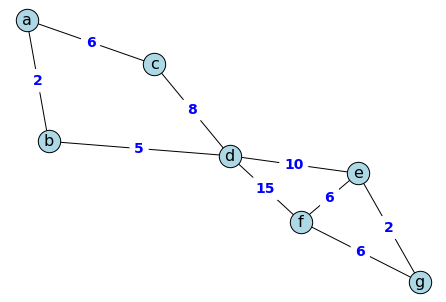
\includegraphics[width=0.7\textwidth]{graph-theory-graphics/dijkstra0.png}
\begin{itemize}
\item We want to find the shortest path from node a to node g
\item Initialize algorithm at node 'a'
\end{itemize}
\end{frame}

\begin{frame}{Example 2: Table to work with}

\begin{columns}
\begin{column}{0.7\textwidth}
\begin{center}

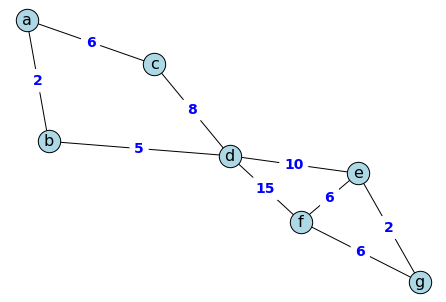
\includegraphics[width=0.7\textwidth]{graph-theory-graphics/dijkstra0.png}



\begin{tabular}{|l|l|l|l|l|l|l|l|}
\hline
current & a & b & c & d & e & f & g \\ \hline
&&&&&&& \\ \hline
&&&&&&& \\ \hline
&&&&&&& \\ \hline
&&&&&&& \\ \hline
&&&&&&& \\ \hline
&&&&&&& \\ \hline
\end{tabular}
\end{center}
\end{column}
\begin{column}{0.3\textwidth}
\begin{enumerate}
\item starting vertex = current, dist = 0.
\item Find all leading to the current vertex. Calculate distances to the start.
\item Mark the current vertex as visited. We will never look at this vertex again.
\item Mark  vertex with  smallest distance as current, and repeat  2.
\end{enumerate}
\end{column}
\end{columns}
\end{frame}

\begin{frame}{Example 2: First Steps}
\begin{columns}
\column{0.4\textwidth}
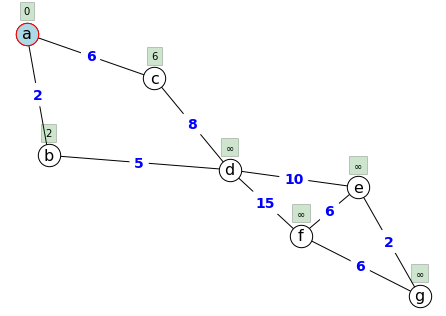
\includegraphics[width=\textwidth]{graph-theory-graphics/dijkstra1.png}
\column{0.6\textwidth}
\begin{tabular}{|l|l|l|l|l|l|l|l|}
\hline
current & a & b & c & d & e & f & g \\ \hline
a & 0 & 2 & 6 & $\infty$ & $\infty$ & $\infty$& $\infty$ \\ \hline
\end{tabular}
\end{columns}
\begin{itemize}
\item Mark a as current, compute distances to adjacent nodes
\end{itemize}
\end{frame}

\begin{frame}{Example 2: Next Steps}
\begin{columns}
\column{0.4\textwidth}
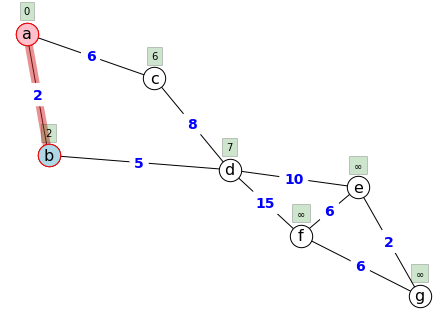
\includegraphics[width=\textwidth]{graph-theory-graphics/dijkstra2.png}
\column{0.6\textwidth}
\begin{tabular}{|l|l|l|l|l|l|l|l|}
\hline
current & a & b & c & d & e & f & g \\ \hline
b & 0 & 2 & 6 & 7 & $\infty$ & $\infty$ & $\infty$ \\ \hline
\end{tabular}
\end{columns}
\begin{itemize}
\item Mark b as current (lowest distance), compute distances
\end{itemize}
\end{frame}

\begin{frame}{Example 2: Later Steps}
\begin{columns}
\column{0.4\textwidth}
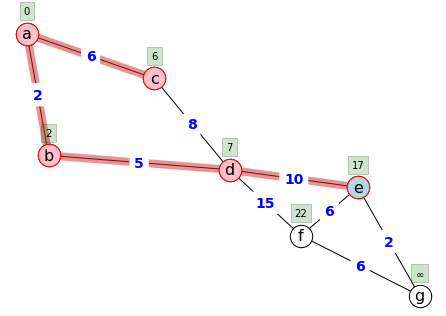
\includegraphics[width=\textwidth]{graph-theory-graphics/dijkstra5.png}
\column{0.6\textwidth}
\begin{tabular}{|l|l|l|l|l|l|l|l|}
\hline
current & a & b & c & d & e & f & g \\ \hline
e & 0 & 2 & 6 & 7 & 17 & 22 & 19 \\ \hline
\end{tabular}
\end{columns}
\begin{itemize}
\item Continue marking vertices as visited and computing distances
\end{itemize}
\end{frame}

\begin{frame}{Example 2: Solution}
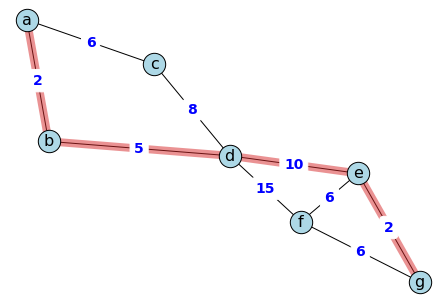
\includegraphics[width=0.7\textwidth]{graph-theory-graphics/dijkstra-soln.png}
\begin{itemize}
\item The shortest path from a to g is a - b - d - e - g
\item Path length = 2 + 5 + 10 + 2 = 19
\end{itemize}
\end{frame}

\begin{frame}{Efficiency of Dijkstra's Algorithm}
\begin{itemize}
\item Dijkstra's algorithm is an \textbf{optimal algorithm}
  \begin{itemize}
  \item It always produces the actual shortest path
  \end{itemize}
\item It is also \textbf{efficient}
  \begin{itemize}
  \item Takes approximately V$^2$ calculations (V = number of vertices)
  \item A graph with 100 vertices: ~10,000 calculations
  \item Fast enough for GPS navigation systems
  \end{itemize}
\item In contrast, listing all possible paths would be \textbf{inefficient}
  \begin{itemize}
  \item 25 vertices could require 10$^{25}$ calculations
  \item World's fastest computer: over 1000 years!
  \end{itemize}
\end{itemize}
\end{frame}

\begin{frame}{Example 3: Shipping Routes}
\begin{itemize}
\item A shipping company needs to find the fastest route from Baltimore to Bakersfield
\item Travel times between processing centers in hours (including 3-hour processing time)
\end{itemize}

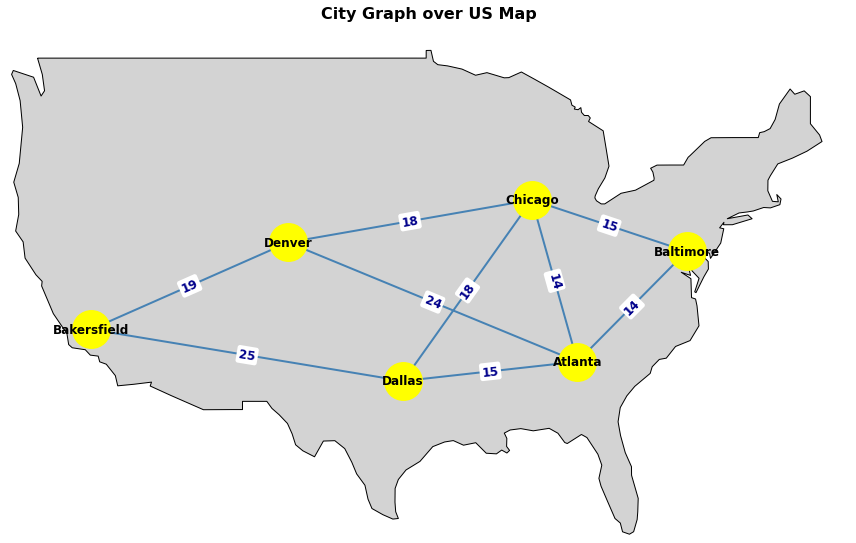
\includegraphics[scale = 0.3]{Figures/graph-us-cities}

\end{frame}

\begin{frame}{Example 3: Shipping Routes - Initialization}

\begin{center}
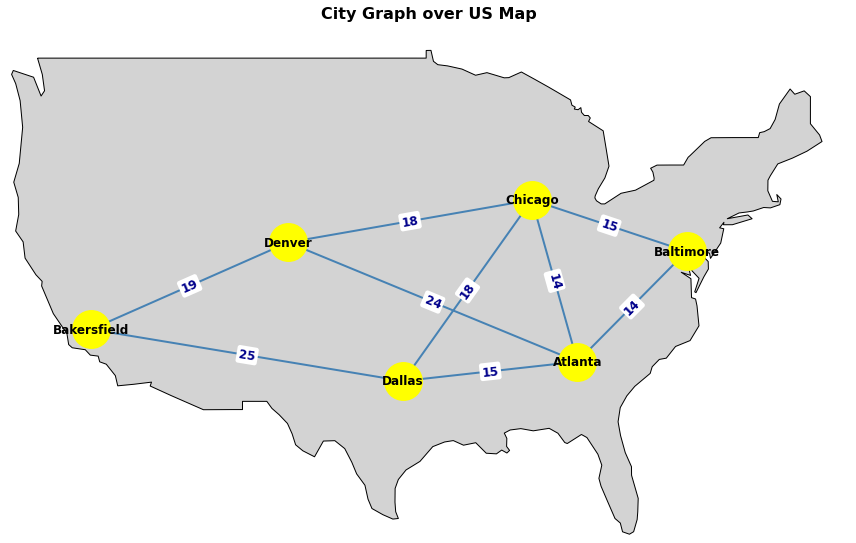
\includegraphics[width = 0.55\textwidth]{Figures/graph-us-cities}
\end{center}
\begin{tabular}{|l|l|l|l|l|l|l|l|}
\hline
current & Baltimore & Chicago & Atlanta & Dallas & Denver & Bakersfield  \\ \hline
Baltimore & 0 & 15 & 14 & $\infty$ & $\infty$ & $\infty$ \\ \hline
&&&&&& \\ \hline
&&&&&& \\ \hline
&&&&&& \\ \hline
&&&&&& \\ \hline
\end{tabular}

\end{frame}






\begin{frame}{Example 3: Shipping Routes - Steps...}

\begin{center}
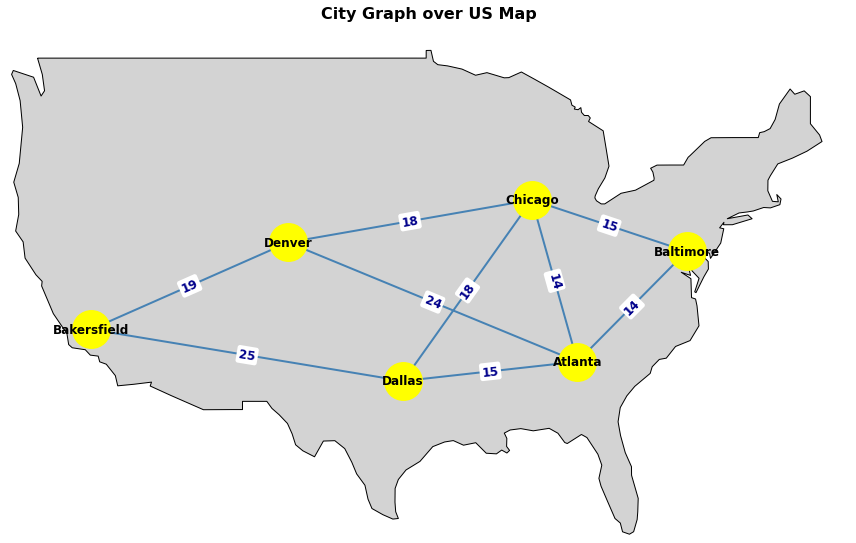
\includegraphics[width = 0.65\textwidth]{Figures/graph-us-cities}
\end{center}
\begin{tabular}{|l|l|l|l|l|l|l|l|}
\hline
current & Baltimore & Chicago & Atlanta & Dallas & Denver & Bakersfield  \\ \hline
&&&&&& \\ \hline
\end{tabular}

\end{frame}

\begin{frame}{Example 3: Shipping Routes - Steps...}

\begin{center}
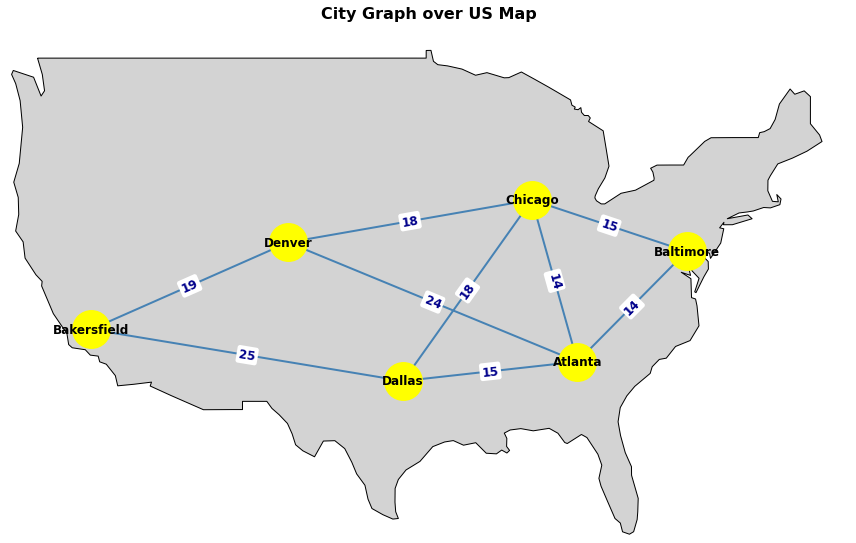
\includegraphics[width = 0.65\textwidth]{Figures/graph-us-cities}
\end{center}
\begin{tabular}{|l|l|l|l|l|l|l|l|}
\hline
current & Baltimore & Chicago & Atlanta & Dallas & Denver & Bakersfield  \\ \hline
&&&&&& \\ \hline
\end{tabular}

\end{frame}



\begin{frame}{Example 3: Shipping Routes - Steps...}

\begin{center}
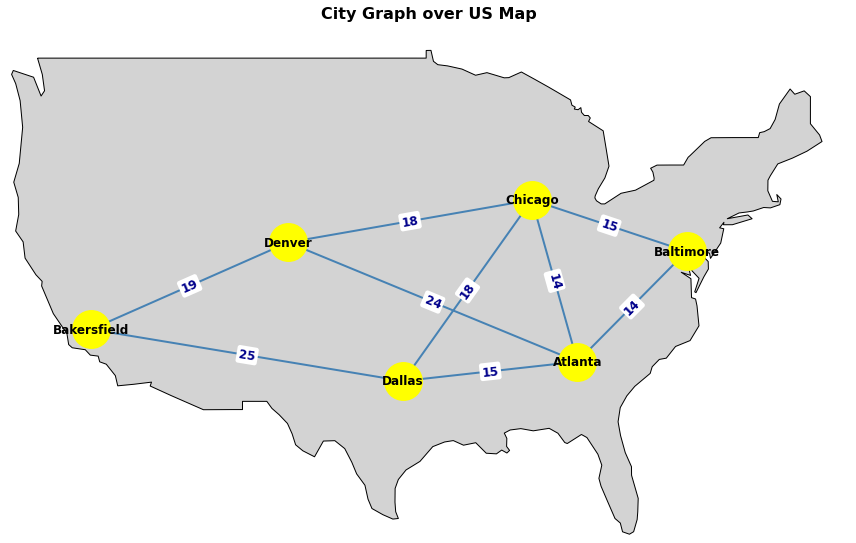
\includegraphics[width = 0.65\textwidth]{Figures/graph-us-cities}
\end{center}
\begin{tabular}{|l|l|l|l|l|l|l|l|}
\hline
current & Baltimore & Chicago & Atlanta & Dallas & Denver & Bakersfield  \\ \hline
&&&&&& \\ \hline
\end{tabular}

\end{frame}






\begin{frame}{Example 3: Shipping Routes}
\begin{itemize}
\item A shipping company needs to find the fastest route from Baltimore to Bakersfield
\item Travel times between processing centers in hours (including 3-hour processing time)
\item We can work directly from a distance table
\end{itemize}

\small
\begin{tabular}{|l|c|c|c|c|c|c|}
\hline
 & Baltimore & Denver & Dallas & Chicago & Atlanta & Bakersfield\\
\hline
Baltimore & * &&&15&14&\\
\hline
Denver &&*&&18&24&19\\
\hline
Dallas&&&*&18&15&25\\
\hline
Chicago &15&18&18&*&14&\\
\hline
Atlanta & 14 & 24&15&14&8&\\
\hline
Bakersfield &&19&25&&&*\\
\hline
\end{tabular}
\end{frame}









\begin{frame}

\begin{tabular}{|l|l|l|l|l|l|l|l|}
\hline
current & Baltimore & Chicago & Atlanta & Dallas & Denver & Bakersfield  \\ \hline
Baltimore & 0 & 15 & 14 & $\infty$ & $\infty$ & $\infty$ \\ \hline
&&&&&& \\ \hline
&&&&&& \\ \hline
&&&&&& \\ \hline
&&&&&& \\ \hline
&&&&&& \\ \hline
&&&&&& \\ \hline
\end{tabular}

\end{frame}

\begin{frame}
\end{frame}

\begin{frame}{Practice Exercise}
Find the shortest path between vertices A and G in this graph:

\begin{center}
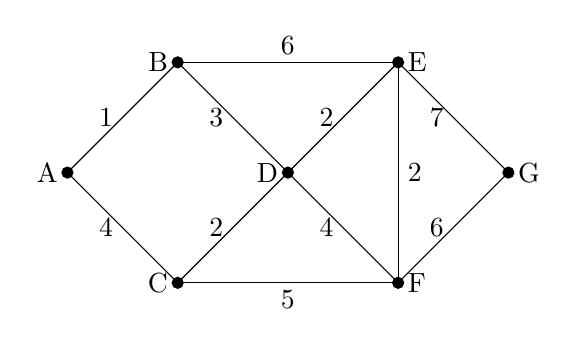
\begin{tikzpicture}[scale=0.7]
\draw[fill] (0,0) circle[radius=.1] node[left]{A};
\draw[fill] (2,2) circle[radius=.1] node[left]{B};
\draw[fill] (2,-2) circle[radius=.1] node[left]{C};
\draw[fill] (4,0) circle[radius=.1] node[left]{D};
\draw[fill] (6,2) circle[radius=.1] node[right]{E};
\draw[fill] (6,-2) circle[radius=.1] node[right]{F};
\draw[fill] (8,0) circle[radius=.1] node[right]{G};
\draw(0,0)--(2,2);
\node at (0.7,1){1};
\draw(0,0)--(2,-2);
\node at (0.7,-1){4};
\draw(2,2)--(4,0);
\node at (2.7,1){3};
\draw(2,-2)--(4,0);
\node at (2.7,-1){2};
\draw(4,0)--(6,2);
\node at (4.7,1){2};
\draw(4,0)--(6,-2);
\node at (4.7,-1){4};
\draw(6,2)--(8,0);
\node at (6.7,1){7};
\draw(6,-2)--(8,0);
\node at (6.7,-1){6};
\draw(2,2)--(6,2);
\node at (4,2.3){6};
\draw(2,-2)--(6,-2);
\node at (4,-2.3){5};
\draw(6,2)--(6,-2);
\node at (6.3,0){2};
\end{tikzpicture}
\end{center}
\end{frame}



\begin{frame}{Software Solutions}
\begin{itemize}
\item NetworkX (Python library)
  \begin{itemize}
  \item Easy graph creation and manipulation
  \item Built-in shortest path algorithms
  \item Visualization capabilities
  \end{itemize}
\item Other options:
  \begin{itemize}
  \item igraph (Python, R, C++)
  \item JUNG (Java)
  \item Graph-tool (Python)
  \item Specialized GIS software for real-world routing problems
  \end{itemize}
\end{itemize}
\end{frame}

\begin{frame}{Summary}
\begin{itemize}
\item Shortest path algorithms find optimal routes between vertices
\item Dijkstra's algorithm:
  \begin{itemize}
  \item Starts at the end vertex (or beginning, in reverse)
  \item Systematically explores the graph
  \item Marks vertices as visited
  \item Always selects the unvisited vertex with the smallest distance
  \end{itemize}
\item It is both optimal and efficient
\item Applications: routing, navigation, network analysis
\end{itemize}
\end{frame}

\end{document}